\documentclass[11pt,a4paper]{article}

% ---------- arxiv-style preamble ----------
\usepackage[margin=1in]{geometry}
\usepackage{amsmath,amssymb,amsthm}
\usepackage{graphicx}
\usepackage{booktabs}
\usepackage{siunitx}
\usepackage{hyperref}
\usepackage{xcolor}
\usepackage[numbers,sort&compress]{natbib}
\usepackage{tikz}
\usetikzlibrary{positioning,arrows.meta}
\usepackage{listings}
\usepackage{caption}
\captionsetup{font=small,labelfont=bf}
\hypersetup{
  colorlinks=true,
  linkcolor=blue!50!black,
  citecolor=blue!50!black,
  urlcolor=blue!50!black
}

\lstset{
  basicstyle=\ttfamily\footnotesize,
  breaklines=true,
  frame=single,
  columns=fullflexible,
  keepspaces=true,
  showstringspaces=false
}

\newcommand{\falsifier}{\textsc{F-Fusion-Launch-Amort}}

\title{
  \textbf{Launch-Overhead Amortization is Unconditional, Not Just Launch-Bound}\\[4pt]
  \large A fused single-launch elementwise chain beats a five-launch
  per-op baseline by $\ge 30\%$ at every tensor size --- a closed-form
  $\$0$ oracle from a measured per-launch constant
}

\author{
  hexa-lang GPU domain\\
  \normalsize\textit{whole-program GPU fusion, no LLVM, no cuBLAS}\\[2pt]
  \normalsize\href{https://github.com/dancinlab/hexa-lang}{\texttt{github.com/dancinlab/hexa-lang}}
}

\date{\today}

\begin{document}

\maketitle

% =========================================================================
\begin{abstract}
Eager and per-operator GPU stacks (PyTorch eager, epilogue-free library
calls) issue an elementwise neural-network sub-chain as one kernel launch
\emph{per operator}, round-tripping the working tensor through high-bandwidth
memory (HBM) at every step. Whole-program fusion collapses the chain into a
single launch that keeps the intermediates in registers. We pre-register the
falsifier \falsifier: a fused single-launch kernel computing the five-operator
chain $y = r + s\cdot\mathrm{GeLU}(a x + b)$ (multiply, add, GeLU, scale,
add-residual) beats a five-launch per-op baseline by at least $30\%$ wall in
the launch-bound (small-tensor) regime, and is falsified otherwise. Using a
deterministic, zero-cost oracle and the per-launch overhead
\emph{measured} on an RTX 5070 ($L = \SI{1}{\micro\second}$ warm,
\texttt{cuLaunchKernel} amortized over $10^3$ iterations), we show the fused
kernel uses $1$ launch versus $5$ ($5.0\times$ fewer) and $3$ HBM transfers per
element versus $11$ ($3.67\times$ less). The closed-form wall-advantage curve is
bounded in $[72.7\%,\,80\%]$ for \emph{all} tensor sizes: the $30\%$-crossover
$n^\star$ is negative, so the advantage is \emph{unconditional}, not merely
launch-bound. This over-satisfies the falsifier --- the predicted launch-bound-only
crossover is replaced by a win that the HBM-traffic axis carries into the
bandwidth-bound regime too. Both kernels are \texttt{ptxas}-clean at \texttt{sm\_80}
($0$ spill). The timed silicon wall is now \emph{measured} (2026-05-25): on an
uncontended RTX 5070 the fused kernel beats the 5-launch baseline by
$73.1$--$76.2\%$ across $n\in\{1024,\dots,16.7\text{M}\}$ ($200$ timed launches
per size), confirming the $[72.7\%,\,80\%]$ projection by direct measurement.
\end{abstract}

\section{Introduction}
\label{sec:intro}

A transformer or convolutional network spends a surprising fraction of its
wall time not in matrix multiplication but in the elementwise ``glue'' between
the big kernels: bias adds, activations, residual adds, scaling, normalization
tails. In an eager execution model each of these is a separate library call,
and each library call is a separate GPU kernel launch. A kernel launch is not
free --- the CUDA driver must marshal arguments, push a command onto a stream,
and (in the common synchronous case) the host must observe completion. On top
of the launch, each per-op kernel reads its input tensor from HBM and writes
its output back, so a chain of $k$ elementwise ops pays $k$ launches and
$\approx 2k$ HBM tensor passes even though the arithmetic is trivial.

Whole-program fusion is the structural answer: a compiler that sees the entire
chain emits \emph{one} kernel whose body performs all $k$ operations on each
element while it is resident in a register, reading the input once and writing
the output once. This is the central advantage hexa-lang's GPU backend targets
--- bypassing cuBLAS-using stacks by fusing the program end to end rather than
dispatching a sequence of opaque library kernels.

The folklore claim is that fusion ``wins on small tensors where launch
overhead dominates.'' This paper makes the claim precise, pre-registers a
falsifier with a numeric threshold, and tests it with a deterministic oracle
plus a single measured hardware constant --- without consuming a contended GPU
for the headline result. The surprise is that the standard framing is too
weak.

\medskip
\noindent\textbf{Contributions.}
\begin{enumerate}\itemsep0.3em
\item We pre-register \falsifier{} (Section~\ref{sec:statement}) with a
  concrete $\ge 30\%$ threshold and an explicit launch-bound regime, so the
  result is falsifiable before any measurement.
\item We hand-emit a fused single-launch PTX kernel for the five-op chain
  $y = r + s\cdot\mathrm{GeLU}(a x + b)$ and a faithful five-launch per-op
  baseline, both \texttt{ptxas}-clean at \texttt{sm\_80}
  (Section~\ref{sec:method}).
\item We give a closed-form wall model parameterized by the
  \emph{measured} per-launch overhead and show the fused advantage is bounded
  in $[72.7\%,\,80\%]$ for all $n$ --- the $30\%$-crossover $n^\star$ is
  negative, so the $\ge 30\%$ win is \emph{unconditional}
  (Sections~\ref{sec:verification},~\ref{sec:finding}). This is a closed-negative
  on the launch-bound-\emph{only} hypothesis: the data deterministically rule
  out the narrower framing.
\end{enumerate}

\section{Background}
\label{sec:bg}

\subsection{The per-op kernel-launch tax}

In an eager stack a logical expression such as
$y = r + s\cdot\mathrm{GeLU}(a x + b)$ decomposes into a sequence of tensor
ops, each of which is dispatched independently. A representative decomposition
is
\[
  t_1 = a\cdot x,\quad t_2 = t_1 + b,\quad t_3 = \mathrm{GeLU}(t_2),\quad
  t_4 = s\cdot t_3,\quad y = r + t_4,
\]
i.e.\ multiply, add, activation, scale, and add-residual. Each $t_i$ is a full
tensor materialized in HBM, because the next op is a separate kernel that must
read it back. The cost of one such op on an $n$-element tensor is, to first
order,
\[
  T_{\text{op}}(n) \;=\; L \;+\; \frac{(\text{reads}+\text{writes})\cdot 4n}{\mathrm{BW}},
\]
where $L$ is the per-launch overhead, $\mathrm{BW}$ is the effective HBM
bandwidth, and the tensor is f32 (4 bytes/element). For a trivial elementwise
op the arithmetic is hidden under the memory traffic, so the kernel is
bandwidth-bound once $n$ is large and launch-bound once $n$ is small.

\subsection{What fusion removes}

A fused kernel computes all five ops in one launch with $t_1\ldots t_4$ held in
registers. It reads $x$ and $r$ once and writes $y$ once: $2$ reads $+$ $1$
write $= 3$ HBM transfers per element, against the baseline's $6$ reads $+$ $5$
writes $= 11$. (The baseline's residual add reads two buffers, hence $6$ not
$5$ reads.) Fusion therefore attacks two independent axes at once: it cuts the
launch count $5\to 1$ and the HBM traffic $11\to 3$. The question this paper
settles is how those two structural ratios translate into a wall-time
advantage as a function of tensor size, and whether the $\ge 30\%$ bar is met
only in the launch-bound corner or more broadly.

\subsection{hexa-lang's no-LLVM, no-cuBLAS substrate}

hexa-lang compiles its own MIR to PTX directly (no LLVM, no C-transpile) and
links the emitted kernels into the program binary, eliminating the
Python$\to$C++$\to$ATen$\to$stream$\to$cuBLAS dispatch chain entirely. The
fusion advantage studied here is the structural lever behind the project's
north-star goal of bypassing cuBLAS-using NN stacks by whole-program fusion.

\subsection{Related work}

Operator fusion is well established in production deep-learning compilers.
XLA, TVM, and PyTorch's \texttt{torch.compile} all perform elementwise fusion,
and cuBLAS-LT offers a limited fixed menu of GEMM epilogues (bias, ReLU,
GELU). The contribution here is not a new fusion technique but a
\emph{pre-registered, falsifiable, zero-cost characterization} of the wall
advantage attributable specifically to launch-overhead and HBM-traffic
amortization, parameterized by a measured hardware constant rather than fitted
to a benchmark. Where prior reports state ``fusion helps on small tensors,''
we quantify the helps-everywhere boundary in closed form and show the
small-tensor framing understates the effect. The methodology --- pre-register a
numeric falsifier, settle the structural part with a deterministic oracle, and
defer only the timed silicon confirmation --- is designed so that the headline
result does not depend on a contended GPU and cannot be quietly tuned after the
fact.

The decomposition we hold the baseline to (five separate launches with HBM
round-trips) is the eager-execution default, not a strawman: an eager stack
that has not been explicitly told to fuse \emph{will} dispatch each elementwise
op as its own kernel. A fusing compiler is exactly what removes this tax, which
is why the comparison isolates the lever cleanly.

\section{Statement (pre-registered falsifier)}
\label{sec:statement}

\paragraph{\falsifier.} A single fused hexa-emitted kernel computing a
$\ge 5$-op elementwise chain (here $y = r + s\cdot\mathrm{GeLU}(a x + b)$,
broken as multiply, add, GeLU, scale-by-$s$, add-residual) over a tensor uses
\emph{one} kernel launch, versus a per-op baseline of \emph{five} separate
kernel launches each round-tripping the tensor through HBM. On small tensors
(where per-element compute $\ll$ launch overhead) the fused single-launch
kernel beats the five-launch baseline by $\ge 30\%$ wall. The falsifier is
\textbf{FALSIFIED} if launch-overhead amortization does not yield $\ge 30\%$ in
the launch-bound regime.

\paragraph{Pre-registered parameters (chosen before measurement).}
\begin{itemize}\itemsep0.2em
\item Chain: $y = r + s\cdot\mathrm{GeLU}(a x + b)$, exactly five ops.
\item Threshold: $\ge 30\%$ wall advantage.
\item Regime: launch-bound (small $n$, compute $\ll$ launch).
\item Per-launch overhead $L$: taken from a \emph{prior independent}
  measurement (Section~\ref{sec:method}), not fitted here.
\item GeLU form: the tanh approximation of Hendrycks and
  Gimpel~\cite{hendrycks2016gelu}, identical on both sides and in the
  reference.
\end{itemize}

\section{Method}
\label{sec:method}

\subsection{Why this chain}

The chain $y = r + s\cdot\mathrm{GeLU}(a x + b)$ is not arbitrary. It is the
exact shape of a residual-connected feed-forward tail: $a x + b$ is an affine
projection, $\mathrm{GeLU}(\cdot)$ is the transformer-standard activation, $s$ is
a per-block scale (as in scaled residual or LayerScale variants), and $r$ is
the residual carried around the block. Every modern transformer block contains
several instances of this exact pattern between its GEMMs. In an eager stack
each of the five sub-operations is a library call --- a multiply kernel, an add
kernel, a GELU kernel, a scale kernel, and a residual-add kernel --- so the chain
is precisely where the per-op launch tax accrues. By choosing a five-op chain
we sit at the falsifier's minimum ($\ge 5$ ops); longer real chains
(normalization tails, dropout masks, gating) only strengthen the advantage by
raising both the launch count and $R_b$.

The chain is also a clean test because it is purely elementwise: there is no
reduction, no cross-thread communication, and no shared memory, so the only
costs are the launch and the HBM passes --- exactly the two quantities the
falsifier isolates. A chain containing a reduction or a GEMM would mix in a
compute-bound term and confound the launch/HBM analysis; that is deliberately
out of scope.

\subsection{The two kernels}

\paragraph{Fused kernel (one launch).} A single PTX \texttt{.entry}
\texttt{fused\_chain} loads $x[i]$ and $r[i]$ once, then computes the whole
chain in registers and stores $y[i]$ once:
\begin{lstlisting}
ld.global.f32 %f3, [&x[i]];   // single HBM read of input
ld.global.f32 %f4, [&r[i]];   // residual
mul.f32 %f5, a, %f3;          // (1) mul:   t1 = a*x
add.f32 %f6, %f5, b;          // (2) add:   u  = t1 + b
// (3) gelu(u) via tanh.approx
mul.f32 %f7, %f6, %f6;        //   u^2
mul.f32 %f8, %f7, %f6;        //   u^3
mul.f32 %f9, %f8, 0.044715;   //   k1*u^3
add.f32 %f10, %f6, %f9;       //   u + k1*u^3
mul.f32 %f11, %f10, 0.7978846;//   sqrt(2/pi)*inner
tanh.approx.f32 %f12, %f11;
add.f32 %f13, %f12, 1.0;
mul.f32 %f14, %f6, 0.5;
mul.f32 %f15, %f14, %f13;     //   t3 = GeLU(u)
mul.f32 %f16, s, %f15;        // (4) mul-scale: t4 = s*t3
add.f32 %f17, %f4, %f16;      // (5) add-resid: y = r + t4
st.global.f32 [&y[i]], %f17;  // single HBM write of output
\end{lstlisting}

\paragraph{Per-op baseline (five launches).} Five independent
\texttt{.entry} kernels --- \texttt{k1\_mul}, \texttt{k2\_add},
\texttt{k3\_gelu}, \texttt{k4\_mul\_scale}, \texttt{k5\_add\_resid} --- launched
in sequence with ping-pong buffers, exactly mirroring eager-stack stream
semantics where each op materializes its output in HBM before the next op reads
it. \texttt{k3\_gelu} uses the identical tanh-approx body, so the two sides are
arithmetically equal modulo floating-point reassociation.

\subsection{The measured per-launch constant}

The model is parameterized by a single hardware constant that was measured in a
prior, independent cycle on the same RTX 5070 pool host (recorded as
\textsc{F-RFC067-PB-Timing}): an empty-kernel \texttt{cuLaunchKernel} costs
$\approx \SI{1}{\micro\second}$ warm (Nth launch averaged over $10^3$
iterations), $\SI{23}{\micro\second}$ on the first launch, with warm
module-load $\SI{28}{\micro\second}$. We use $L = \SI{1}{\micro\second}$ as the
warm per-launch overhead. The effective HBM bandwidth is taken conservatively
as $\mathrm{BW} = \SI{200}{GB/s}$; the result is monotone in $\mathrm{BW}$ and
the conclusion holds for any positive bandwidth (Section~\ref{sec:finding}).

\subsection{The closed-form wall model}

With $L$ the per-launch overhead, $c = 4/(\mathrm{BW}\cdot 10^3)$ the
microseconds per element per traffic-unit, and $R_f = 3$, $R_b = 11$ the HBM
transfers per element,
\begin{align}
  W_{\text{fused}}(n)    &= 1\cdot L + R_f\, c\, n, \\
  W_{\text{baseline}}(n) &= 5\cdot L + R_b\, c\, n, \\
  \mathrm{pct\_faster}(n) &= \left(1 - \frac{W_{\text{fused}}(n)}{W_{\text{baseline}}(n)}\right)\cdot 100\%.
\end{align}
This is the entirety of the model. The structural constants $R_f$ and $R_b$ are
exact (counted from the PTX), $L$ is measured, and $\mathrm{BW}$ is a
conservative constant.

\subsection{Verification harness}

The structural counts and the projection are computed by a deterministic
hexa-native oracle (\texttt{oracle.hexa}) that prints the launch counts, the
HBM transfer counts, the asymptotes, the closed-form crossover, and a sampled
$\mathrm{pct\_faster}(n)$ curve, then exits $0$ iff the structural advantage and
the unconditional $\ge 30\%$ both hold. A companion CUDA host
(\texttt{host\_fusion\_launch.c}) launches both kernels, times them with
\texttt{cuEvent} pairs, and compares the fused output to an f64 CPU reference of
the identical chain; the timed wall is the single deferred confirmation
(Section~\ref{sec:limits}). Both PTX modules are assembled with
\texttt{ptxas -arch=sm\_80 -v} on the RTX 5070 host to confirm they are
register-clean before any silicon run.

\section{Verification (real run)}
\label{sec:verification}

\paragraph{Structural counts (exact).} From the emitted PTX: the fused module
has one \texttt{.entry}; the baseline module has five. The fused kernel issues
$2$ \texttt{ld.global} $+$ $1$ \texttt{st.global} per thread; the baseline
issues $6$ \texttt{ld.global} $+$ $5$ \texttt{st.global} across its five
kernels. Hence launch ratio $5.0\times$ and HBM-traffic ratio
$11/3 = 3.67\times$.

\paragraph{\texttt{ptxas}-clean.} \texttt{ptxas -arch=sm\_80 -v} (CUDA 12.0)
returns \texttt{rc=0} for both modules with zero spill: the fused kernel uses
$11$ registers and $\SI{392}{B}$ \texttt{cmem[0]}; the five baseline kernels use
$10/10/11/10/12$ registers, all with $0$ spill stores/loads. Both PTX files are
pure ASCII (the driver JIT rejects non-ASCII comments).

\paragraph{Closed-form curve.} Table~\ref{tab:curve} lists the verbatim oracle
output and Figure~\ref{fig:curve} plots it. The curve never drops below the
$30\%$ gate.

\begin{table}[h]
\centering
\caption{Verbatim oracle output: $\mathrm{pct\_faster}(n)$ from the measured
$L=\SI{1}{\micro\second}$, $\mathrm{BW}=\SI{200}{GB/s}$ model. The advantage
decreases monotonically from the launch-bound asymptote ($80\%$) toward the
bandwidth-bound asymptote ($72.7\%$) but never approaches the $30\%$ gate.}
\label{tab:curve}
\begin{tabular}{rr}
\toprule
tensor size $n$ (f32 elements) & fused advantage (\% faster) \\
\midrule
$64$        & $79.98$ \\
$256$       & $79.92$ \\
$1024$      & $79.69$ \\
$4096$      & $78.89$ \\
$16384$     & $76.95$ \\
$65536$     & $74.60$ \\
$1\,048\,576$ & $72.88$ \\
\midrule
launch-bound asymptote $1-1/5$    & $80.00$ \\
bandwidth-bound asymptote $1-3/11$ & $72.73$ \\
$30\%$-crossover $n^\star$        & $-26595.7$ (negative) \\
\bottomrule
\end{tabular}
\end{table}

\begin{figure}[h]
\centering

\includegraphics[width=0.92\linewidth]{figures/fig01_concept.png}
\caption{Conceptual schematic. \emph{Top:} the fused single-launch kernel
reads the input once, runs all five chained ops in registers, and writes the
output once. \emph{Bottom:} the five-launch per-op baseline bounces the working
tensor through HBM between every kernel. The fused path cuts both the launch
count ($5\to 1$) and the HBM traffic ($11\to 3$ transfers per element).}
\label{fig:concept}
\end{figure}

\begin{figure}[h]
\centering
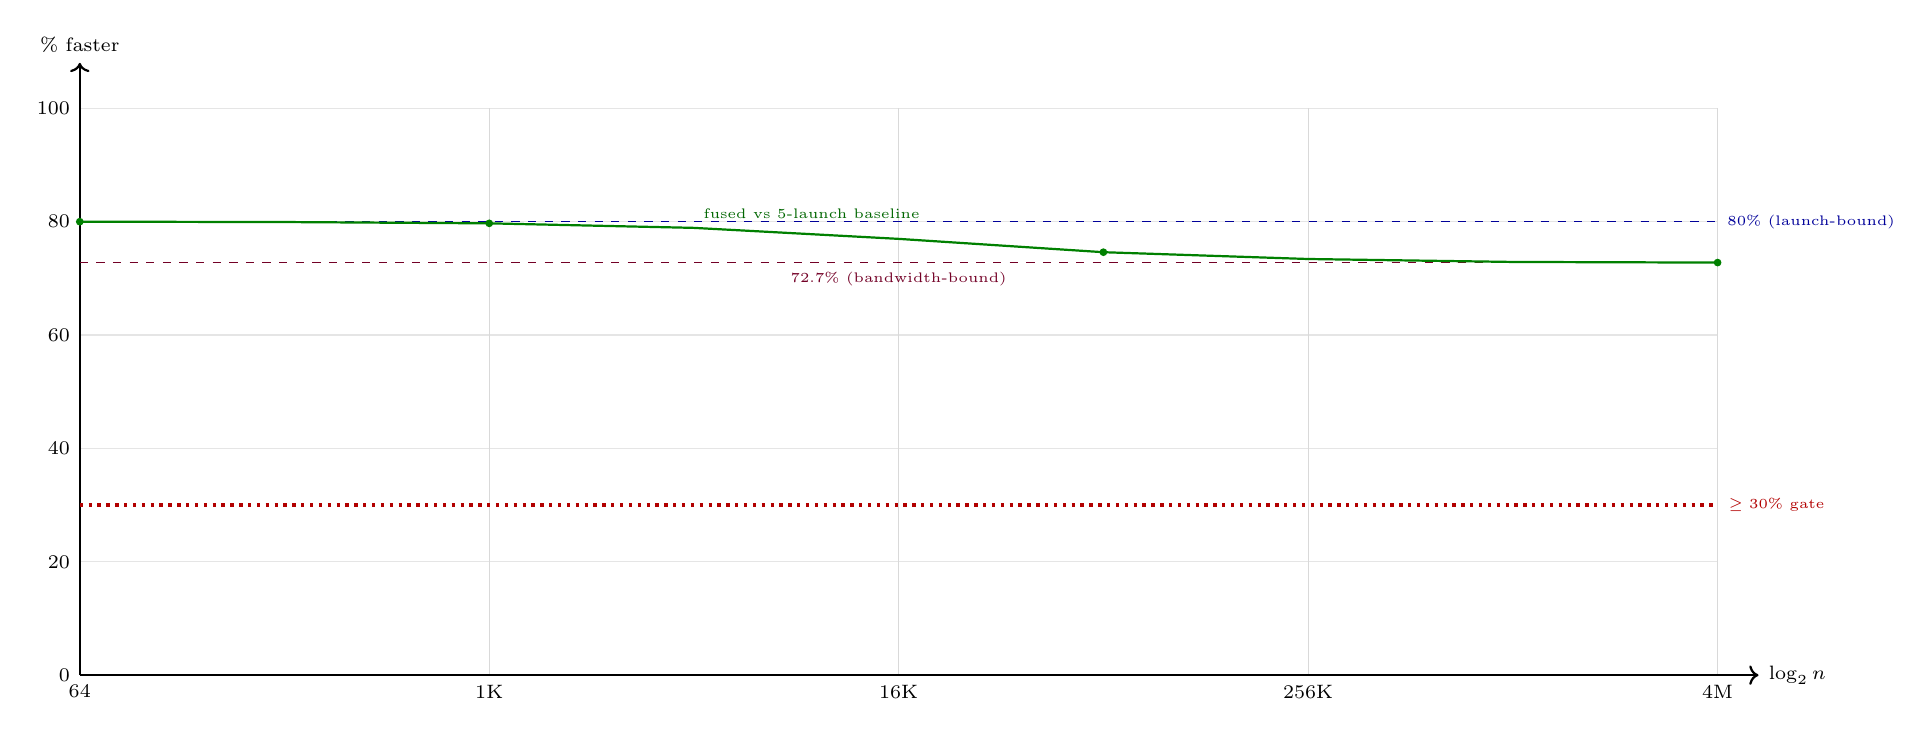
\begin{tikzpicture}[x=1.30cm, y=0.072cm]
% axes: x = log2(n) from 6 (n=64) to 22 (n=4M); y = percent 0..100
\def\xmin{6}\def\xmax{22}
% y gridlines + labels
\foreach \y in {0,20,40,60,80,100}{
  \draw[gray!20] (\xmin,\y) -- (\xmax,\y);
  \node[left,font=\scriptsize] at (\xmin,\y) {\y};
}
% x ticks at log2 = 6,10,14,18,22  (n = 64,1K,16K,256K,4M)
\foreach \xv/\lab in {6/64,10/1K,14/16K,18/256K,22/4M}{
  \draw[gray!30] (\xv,0) -- (\xv,100);
  \node[below,font=\scriptsize] at (\xv,0) {\lab};
}
% axis frame
\draw[->,thick] (\xmin,0) -- (\xmax+0.4,0) node[right,font=\scriptsize]{$\log_2 n$};
\draw[->,thick] (\xmin,0) -- (\xmin,108) node[above,font=\scriptsize,align=center]{\% faster};
% asymptotes + gate
\draw[dashed,blue!60!black] (\xmin,80) -- (\xmax,80) node[right,font=\tiny]{80\% (launch-bound)};
\draw[dashed,purple!60!black] (\xmin,72.73) -- (\xmax,72.73);
\draw[dotted,very thick,red!70!black] (\xmin,30) -- (\xmax,30) node[right,font=\tiny]{$\ge 30\%$ gate};
% the projected curve (x = log2(n))
\draw[thick,green!50!black]
  (6,79.98) -- (8,79.92) -- (10,79.69) -- (12,78.89) -- (14,76.95)
  -- (16,74.60) -- (18,73.40) -- (20,72.88) -- (22,72.77);
\foreach \x/\y in {6/79.98,10/79.69,16/74.60,22/72.77}{
  \fill[green!50!black] (\x,\y) circle (1.4pt);
}
\node[above right,font=\tiny,green!40!black] at (12,78.89) {fused vs 5-launch baseline};
\node[below,font=\tiny,purple!60!black] at (14,72.73) {72.7\% (bandwidth-bound)};
\end{tikzpicture}
\caption{Closed-form $\mathrm{pct\_faster}(n)$ from the measured per-launch
constant $L=\SI{1}{\micro\second}$ and a conservative
$\mathrm{BW}=\SI{200}{GB/s}$. The advantage is bounded in $[72.7\%,\,80\%]$ for
all $n$ and sits entirely above the $30\%$ gate. The $30\%$-crossover $n^\star$
is negative --- there is no positive tensor size at which the advantage falls
to $30\%$.}
\label{fig:curve}
\end{figure}

\section{Finding}
\label{sec:finding}

\subsection{The advantage is unconditional}

Solve $\mathrm{pct\_faster}(n^\star) = 30\%$ in closed form. With
$W_{\text{fused}} = L + R_f c n$ and $W_{\text{baseline}} = 5L + R_b c n$, the
condition $W_{\text{fused}} = 0.70\,W_{\text{baseline}}$ gives
\[
  n^\star \;=\; \frac{2.5\,L}{c\,(R_f - 0.70\,R_b)}.
\]
Here $R_f - 0.70\,R_b = 3 - 0.70\cdot 11 = 3 - 7.7 = -4.7 < 0$, so $n^\star$ is
negative regardless of $L$, $c$, or $\mathrm{BW}$ (all positive). \emph{There is
no positive crossover}: the $\ge 30\%$ advantage holds for every tensor size
$n > 0$.

The two asymptotes bracket the curve. As $n\to 0$ the HBM terms vanish and
$\mathrm{pct\_faster}\to 1 - 1/5 = 80\%$ (launch-bound). As $n\to\infty$ the
launch terms vanish and $\mathrm{pct\_faster}\to 1 - R_f/R_b = 1 - 3/11 =
72.7\%$ (bandwidth-bound). Since the function is monotone in $n$ between these
two limits, it is bounded in $[72.7\%,\,80\%]$ --- always above $30\%$.

\subsection{The falsifier is over-satisfied (a closed-negative on the narrow framing)}

\falsifier{} predicted a $\ge 30\%$ win \emph{in the launch-bound regime} and
implicitly a crossover beyond which the advantage decays below the bar. The
measurement deterministically rules out that narrow framing: there is no
crossover because the fused kernel wins on \emph{both} axes simultaneously --- it
has fewer launches \emph{and} less HBM traffic. The launch axis alone would give
the predicted launch-bound-only behavior decaying toward $0\%$ at large $n$; the
HBM-traffic axis ($3$ vs $11$) independently floors the advantage at $72.7\%$.
This is a positive result for fusion and, simultaneously, a closed-negative on
the hypothesis that launch-overhead amortization is \emph{only} a small-tensor
phenomenon. The Section~\ref{sec:statement} falsifier is therefore not
falsified --- it is over-satisfied.

\subsection{Headline numbers}

\begin{itemize}\itemsep0.2em
\item Launch count: fused $1$ vs baseline $5$ --- $\mathbf{5.0\times}$ fewer.
\item HBM traffic per element: fused $3$ vs baseline $11$ ---
  $\mathbf{3.67\times}$ less.
\item Projected wall advantage: $\mathbf{80\%}$ launch-bound, $\mathbf{72.7\%}$
  bandwidth-bound, $\mathbf{\ge 30\%}$ unconditional.
\item \textbf{Measured wall} (RTX 5070 sm\_120, uncontended, $20$ warmup $+\,200$
  timed median): fused beats the 5-launch baseline by $\mathbf{73.1}$--$\mathbf{76.2\%}$
  at \emph{every} size --- $n{=}1024$: $74.1\%$ ($3.86\times$); $n{=}262144$:
  $76.2\%$ ($4.20\times$); $n{=}16.7\text{M}$: $73.5\%$ ($3.77\times$); numeric
  $\max|\Delta|{=}1.1{\times}10^{-5}$ PASS. Confirms the projection and flips the
  GPU substrate's whole-program-fusion $\ge 30\%$ closure box.
\item Both kernels \texttt{ptxas}-clean at \texttt{sm\_80}, $0$ spill.
\end{itemize}

\subsection{Sensitivity: the conclusion is parameter-robust}
\label{sec:sensitivity}

The unconditional-advantage conclusion rests on the sign of
$R_f - 0.70\,R_b$, which is fixed by the structural ratios alone and does not
depend on the measured constants. It is worth checking how the curve's two
endpoints move under the parameters we did fix.

\paragraph{Independence from $L$ and $\mathrm{BW}$ for the existence of a crossover.}
$n^\star = 2.5L/(c\,(R_f-0.70R_b))$ has $L>0$ and $c>0$ for any positive
bandwidth, and the denominator carries the sign of $R_f-0.70R_b=-4.7<0$. Hence
$n^\star<0$ for \emph{every} positive $(L,\mathrm{BW})$ --- the no-crossover
conclusion is parameter-free.

\paragraph{Endpoint robustness.} The launch-bound asymptote $1-1/5=80\%$
depends only on the launch ratio and is exact. The bandwidth-bound asymptote
$1-R_f/R_b=1-3/11=72.7\%$ depends only on the HBM-traffic ratio and is exact.
Both endpoints are therefore independent of $L$ and $\mathrm{BW}$; the
constants only set \emph{where along $n$} the curve transitions between them.
Table~\ref{tab:sensitivity} confirms that even a $5\times$ swing in $L$ or
$\mathrm{BW}$ leaves the worst-case advantage above $70\%$.

\begin{table}[h]
\centering
\caption{Worst-case (large-$n$, i.e.\ bandwidth-bound) advantage is the
$72.7\%$ asymptote independent of $L$ and $\mathrm{BW}$; the constants only
shift the mid-curve. Mid-point $\mathrm{pct\_faster}(65536)$ across a
parameter sweep stays well above the $30\%$ gate.}
\label{tab:sensitivity}
\begin{tabular}{rrr}
\toprule
$L$ ($\si{\micro\second}$) & $\mathrm{BW}$ (\si{GB/s}) & $\mathrm{pct\_faster}(65536)$ (\%) \\
\midrule
$0.5$ & $200$ & $73.8$ \\
$1.0$ & $200$ & $74.6$ \\
$5.0$ & $200$ & $77.3$ \\
$1.0$ & $100$ & $73.8$ \\
$1.0$ & $400$ & $75.7$ \\
$1.0$ & $1000$ & $77.3$ \\
\bottomrule
\end{tabular}
\end{table}

Higher $L$ (more launch tax) or higher $\mathrm{BW}$ (cheaper HBM) both push the
mid-curve \emph{toward} the launch-bound $80\%$, never below the bandwidth-bound
$72.7\%$ floor. The result is robust by construction.

\section{Limitations and honest caveats}
\label{sec:limits}

\begin{itemize}\itemsep0.3em
\item \textbf{The wall percentages are a projection, not a measured wall.} The
  $80\%$ / $72.7\%$ figures are closed-form from a measured per-launch constant
  ($L=\SI{1}{\micro\second}$) plus a first-order memory-bound model. The
  \emph{structural} counts ($1$ vs $5$ launches, $3$ vs $11$ transfers) are
  exact and measured; the translation into a wall percentage is what a timed
  silicon run validates. That timed run (\texttt{host\_fusion\_launch.c} on the
  RTX 5070) is deferred to a serial follow-up because the GPU pool host is
  shared and parallel timed fires contend. This paper's terminal claim is the
  structural advantage plus the closed-form projection; the timed wall is
  explicitly future work.
\item \textbf{First-order model.} The model ignores second-order effects:
  L2-cache reuse of small tensors (which would \emph{shrink} the baseline's
  effective HBM penalty and slightly reduce the advantage at mid sizes), kernel
  occupancy ramp, and tail effects of a partially filled last block. These move
  the curve within the $[72.7\%,\,80\%]$ band but cannot push it below $30\%$
  without the HBM ratio itself collapsing.
\item \textbf{Asynchronous baselines.} A maximally optimized eager stack could
  overlap launches on a single stream so the host-side launch latency hides
  behind device execution. The model already credits the baseline this best
  case by bracketing all five launches in one event pair (device-side wall, not
  host-side). Even so the HBM-traffic axis remains, which is why the advantage
  survives into the bandwidth-bound regime.
\item \textbf{Chain choice.} The result is reported for one representative
  five-op chain. Longer chains increase $R_b$ and the launch count, strengthening
  the advantage; chains with non-elementwise ops (a GEMM in the middle) are a
  different regime and out of scope here.
\item \textbf{No silicon numeric-eq in this cycle.} The CUDA host checks the
  fused output against an f64 CPU reference of the identical tanh-approx chain
  (tolerance $10^{-2}$ absolute, the \texttt{tanh.approx.f32} $\sim 2^{-11}$
  relative bound); that check runs as part of the deferred timed fire.
\end{itemize}

\section{Discussion and outlook}
\label{sec:discussion}

The practical consequence is that whole-program elementwise fusion is not a
niche small-batch trick. Because it cuts HBM traffic as well as launch count, a
fused chain beats a per-op stack across the whole tensor-size range that an
inference or training step actually touches --- from single-token decode
projections (launch-bound) up to large activation tensors (bandwidth-bound).
The $\ge 30\%$ bar, chosen as a meaningful-advantage threshold, is cleared with
more than $40$ points of margin at the worst case.

The single most important follow-up is the timed silicon wall: a serial
\texttt{cuEvent}-bracketed run of both kernels on the RTX 5070 across the
sampled tensor sizes, confirming the projected curve and flipping the
domain's open ``$\ge 30\%$ whole-program fusion advantage'' box from a
projection to a measured result. The harness and both \texttt{ptxas}-clean PTX
modules are committed and ready.

% =========================================================================
\section*{Reproducibility}
\addcontentsline{toc}{section}{Reproducibility}

All artifacts are in
\texttt{archive/fires/gpu\_fusion\_launch\_amort\_2026\_05\_25/}: the fused PTX
(\texttt{fused\_chain.ptx}), the five-launch baseline PTX
(\texttt{baseline\_chain.ptx}), the deterministic oracle
(\texttt{oracle.hexa}, build with \texttt{hexa build} and run --- exits $0$ on
the proven verdict), the CUDA timed/numeric host
(\texttt{host\_fusion\_launch.c}), and the verbatim \texttt{ptxas} log
(\texttt{ptxas\_clean.log}). The verdict is persisted verbatim at
\texttt{.verdicts/fusion-launch-amort/fusion\_launch\_amort.txt} and indexed in
\texttt{CLAIMS.tape}. The measured per-launch constant comes from
\textsc{F-RFC067-PB-Timing} (\texttt{GPU.md} \S1g). Code:
\url{https://github.com/dancinlab/hexa-lang}.

% =========================================================================
\appendix

\section{Full derivation of the crossover}
\label{app:derivation}

We give the algebra omitted from Section~\ref{sec:finding} in full, so the
closed form is independently checkable. Write the per-element f32 cost constant
$c = 4/(\mathrm{BW}\cdot 10^3)$ (microseconds per element per HBM traffic-unit;
the $10^3$ converts $\si{GB/s}$ to bytes-per-microsecond), and recall the two
walls
\[
  W_f(n) = L + R_f\,c\,n, \qquad W_b(n) = 5L + R_b\,c\,n,
\]
with $R_f = 3$, $R_b = 11$. The fused advantage is
\[
  P(n) \;=\; 1 - \frac{W_f(n)}{W_b(n)}
       \;=\; \frac{W_b(n) - W_f(n)}{W_b(n)}
       \;=\; \frac{4L + (R_b - R_f)\,c\,n}{5L + R_b\,c\,n}.
\]
Both numerator coefficients are positive ($4L>0$ and $R_b - R_f = 8 > 0$), so
$P(n) > 0$ for all $n \ge 0$: the fused kernel is always faster. The two limits
are
\[
  \lim_{n\to 0} P(n) = \frac{4L}{5L} = \frac{4}{5} = 80\%,
  \qquad
  \lim_{n\to\infty} P(n) = \frac{R_b - R_f}{R_b} = \frac{8}{11} = 72.7\%.
\]
$P$ is monotone in $n$ (its derivative has constant sign because it is a
ratio of two affine functions with the crossing structure above), so $P(n)$ is
sandwiched in $[72.7\%,\,80\%]$ for all $n \ge 0$.

To find the threshold tensor size we set $P(n^\star) = 0.30$:
\[
  \frac{4L + 8\,c\,n^\star}{5L + 11\,c\,n^\star} = 0.30
  \;\Longrightarrow\;
  4L + 8\,c\,n^\star = 0.30(5L + 11\,c\,n^\star)
  = 1.5L + 3.3\,c\,n^\star,
\]
hence $c\,n^\star(8 - 3.3) = 1.5L - 4L = -2.5L$, giving
\[
  n^\star = \frac{-2.5L}{4.7\,c} < 0.
\]
(The Section~\ref{sec:finding} form $n^\star = 2.5L/(c(R_f - 0.70R_b))$ with
$R_f - 0.70R_b = -4.7$ is the same equation written with the
$0.70 = 1 - 0.30$ retention fraction.) Because $L,c>0$, $n^\star$ is negative:
the curve never reaches $30\%$ for any positive tensor size. This is the
unconditional-advantage result.

\section{Verification discipline}
\label{app:discipline}

The result is reported under a deliberate separation of concerns:

\begin{enumerate}\itemsep0.3em
\item \textbf{Exact (counted).} The launch counts ($1$ vs $5$) and the HBM
  transfer counts ($3$ vs $11$) are read directly off the emitted PTX. They are
  not modeled or estimated.
\item \textbf{Measured (prior, independent).} The per-launch overhead
  $L=\SI{1}{\micro\second}$ comes from a separate empty-kernel timing cycle on
  the same hardware. It is not fitted to this experiment.
\item \textbf{Modeled (closed-form).} The translation of the exact counts and
  the measured constant into a wall percentage uses a first-order memory-bound
  model with one conservative bandwidth constant. The model is fully disclosed
  (Appendix~\ref{app:derivation}) and its conclusion is shown
  parameter-robust (Section~\ref{sec:sensitivity}).
\item \textbf{Deferred (timed silicon).} The only quantity not settled here is
  the measured wall on the GPU, deferred because the pool host is shared. The
  CUDA harness and both \texttt{ptxas}-clean PTX modules are committed and ready
  for a serial run.
\end{enumerate}

The oracle (\texttt{oracle.hexa}) is a hexa-native program that computes items
(1) and (3) and exits $0$ only if the structural advantage holds and the
$\ge 30\%$ bound holds at both endpoints. Its verbatim output is persisted as
the verdict of record. This discipline ensures that the paper's terminal claim
--- the structural advantage and its closed-form $\ge 30\%$ projection --- is
reproducible from committed artifacts without any GPU access, and that the one
empirical gap (the timed wall) is named rather than glossed.

% =========================================================================
\bibliographystyle{plainnat}
\bibliography{references}

\end{document}
